
%%%%%%%%%%%%%%%%% Introduction to the Assignment %%%

In this Assignment, \textit{\textbf{Problem 4 - Pulse modulation techniques and observations of the atmosphere}}, ...


%%%%%%%%%%%%%%%%% TASK 1 %%%
\section{Pulse coding techniques}
By studying the auto correlation and ambiguity functions, one can compare different pulse coding techniques and determine the best suitable pulse coding technique for a given application.

\subsection{Normalized ambiguity diagram}
\begin{figure}[h!]
	\centering
	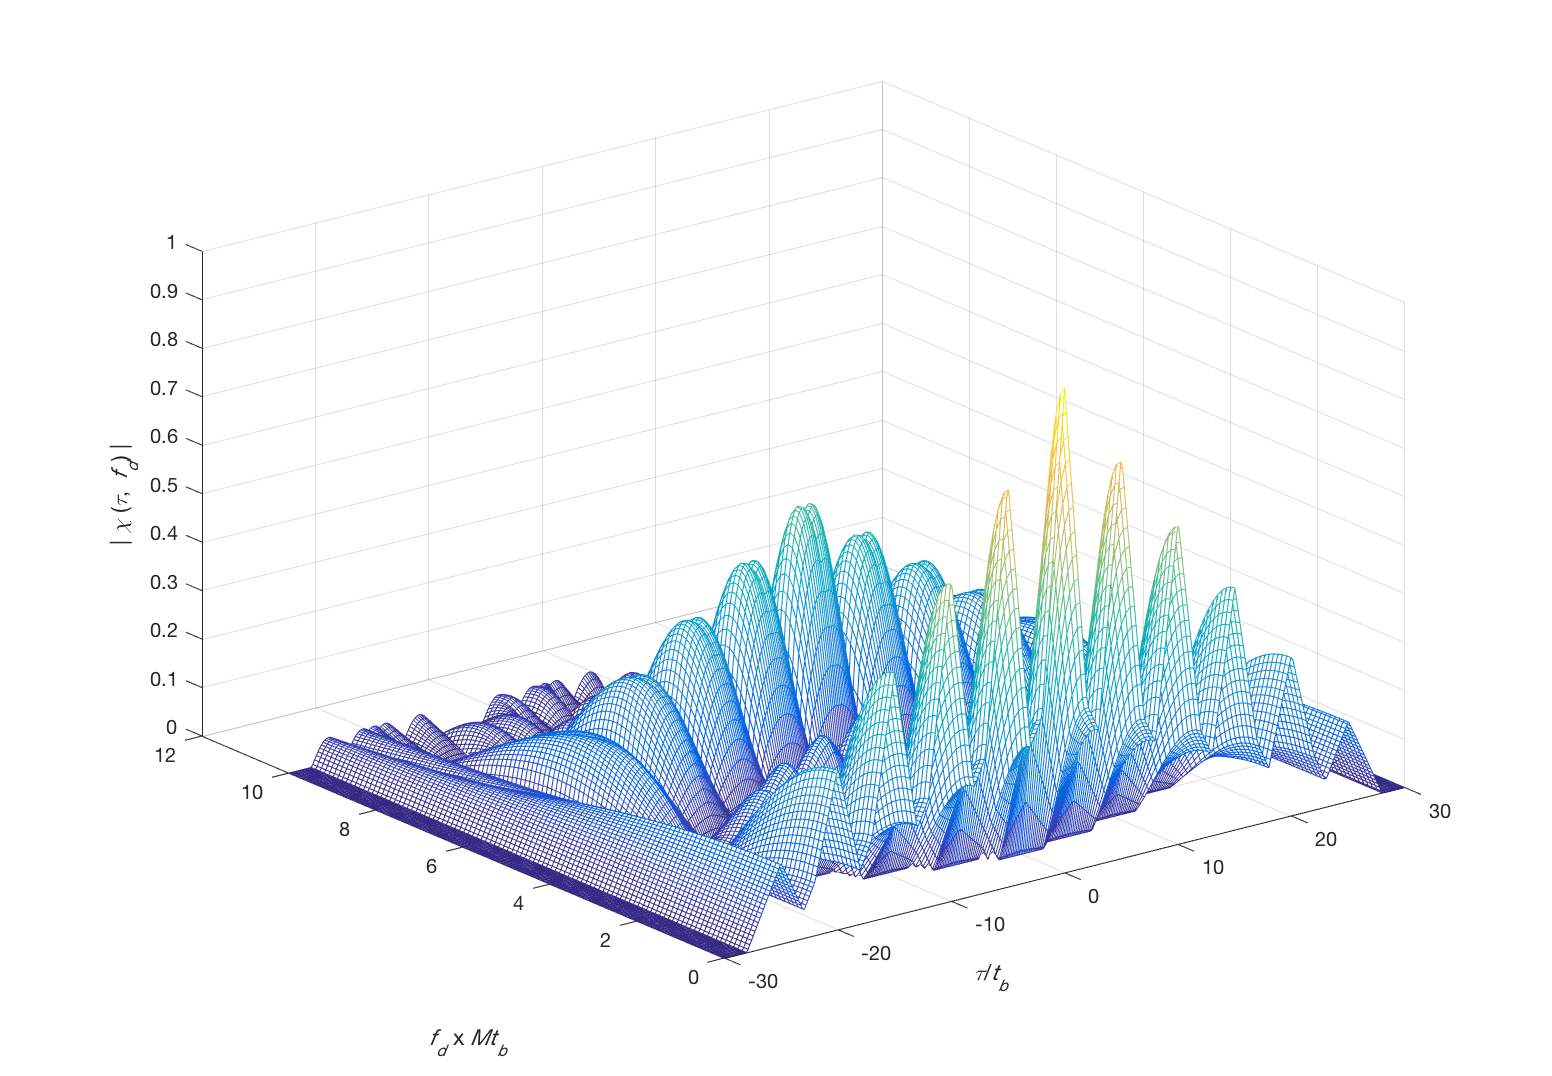
\includegraphics[width=0.9\textwidth]{images/ass1_1_AmbDiag_PulseTrain}
	\caption{Normalized Ambiguity Diagram for a 6-pulse train}
	\label{fig:ambdiag1}
\end{figure}
In the given assignment program the plotted diagram (e.g. \ref{fig:ambdiag1}) is normalized on all three axes.
The axes are the ambiguity function in z-direction, Doppler in x-direction and Delay in y-direction. In the plot of Fig. \ref{fig:ambdiag1}, the negative Doppler positive delay part was shifted to positive Doppler negative delay, which is why the x-axis has no negative numbers. This can be done because of the symmetry of the ambiguity function.\\
The doppler and delay are normalized to the number of sample. \todo{check that! check also wikipedia on normalised frequency}

If the axes would not be normalized, the x- and y-axis would be labelled with $f_d$ and $\tau$, respectively, with units of Hertz and seconds. Since the ambiguity function is normalized w.r.t. the delay and doppler frequency, the z-axis will not change. \todo{really? see Matlabbook chap 4 eq. 4.10. Is z-axis normalized to amplitude?}

\subsection{Amplitude normalized auto-correlation function}
According to \todo{add matlabbook reference} the auto-correlation function can be obtained by $\chi(\tau,0)$. \todo{think that's not true, because thats 1- tau over t, where's the amplitude in here?}
\todo{also, might check richards chapter 20, pdf page 838}


\subsection{Radar system properties}
\label{subsec:props}
\begin{enumerate}
	\item \textbf{Range resolution}\\
			Range resolution describes a specific area or spatial extent in which two distinct objects can be distinguished from each other. It is denoted as
			\begin{equation}
				\Delta R = \frac{\tau c}{2}
			\end{equation}
			Objects that are separated by a distance larger than $\Delta R$ can be distinguished from each other, otherwise they are not.
			Range resolution can be improved by decreasing the SNR or the pulse width $T_p$, which means increasing the Bandwidth, denoted as $BW = \frac{1}{T_p}$. Increasing the Bandwidth can be done by modulating the signal in some form.
			\begin{equation}
				\Delta R = \frac{c}{2 BW}
			\end{equation}
	\item \textbf{Frequency resolution}\\
			According to Curry, chap. 8.9 \citep{radarSystemPerformance} doppler frequency resolution is about equal to the reciprocal of the pulse length. 
			\begin{equation}
				f_r = \frac{1}{T_p}
			\end{equation}
			Thus, the Doppler frequency resolution gets better, the greater the pulse length is, which is again coupled to reduction of range resolution.
	\item \textbf{Doppler tolerance} \\
			According to Richards et al.\citep{richards2010principles} Doppler tolerance describes the response of the waveform in the presence of an uncompensated Doppler. This means, doppler tolerance defines a maximum for Doppler shift so that the matched filter can provide a high enough correlation peak compared to the noise.
	\item \textbf{Ambiguities} \\
			A range ambiguity can occur, when the interpulse period (IPP) is shorter than the round-trip travel time to the target. This would show up as a closer target in the next pulse period, where one could not distinguish anymore if it's a close or distant target.\\
			Frequency ambiguities \todo{doppler frequency? depending on the sampling?}
			
\end{enumerate}

\subsection{Detectability}
Detectability of a target can be increased by integrating multiple samples coherently. Here, the signal adds up in phase, but uncorrelated clutter and noise does not add up in phase, effectively leading to a higher Signal-to-Clutter and Signal-to-Noise ratio \citep{richards2010principles}.

\subsection{Properties of the ambiguity function}
The ambiguity function is a 2D function of time delay $\tau$ and Doppler frequency. In general, the ambiguity function shows, how the received signal is distorted by the matched filter, means how the matched filter responds to the received signal, when the Doppler shift is not compensated by the receiving system \citep{richards2010principles}. The three-dimensional representation of the ambiguity function is usually normalized to unit energy (e.g. to the peak of the received signal), to allow comparison. While there exist different notations of the ambiguity functions, a common one can be seen in formula \ref{eq:AF}.

\begin{equation}
	\chi(\tau,f_d) = \int_{-\infty}^\infty s(t)*s(t-\tau)e^{j2\pi f_dt}dt
	\label{eq:AF}
\end{equation}

As already stated in chapter \ref{subsec:props}, the range resolution can be increased by increasing the Bandwidth, respectively decreasing the pulse width. Both these components happen to be in complementary coding, where the pulses are relatively short, and those pulses are phase coded which increases the Bandwidth. Fig. \ref{fig:complCoding3D} and \ref{fig:complCodingProps} show such a complementary phase coded pulse with a code length of 8.

\begin{figure}[!htbp]
  \centering
  \begin{minipage}[b]{0.45\textwidth}
    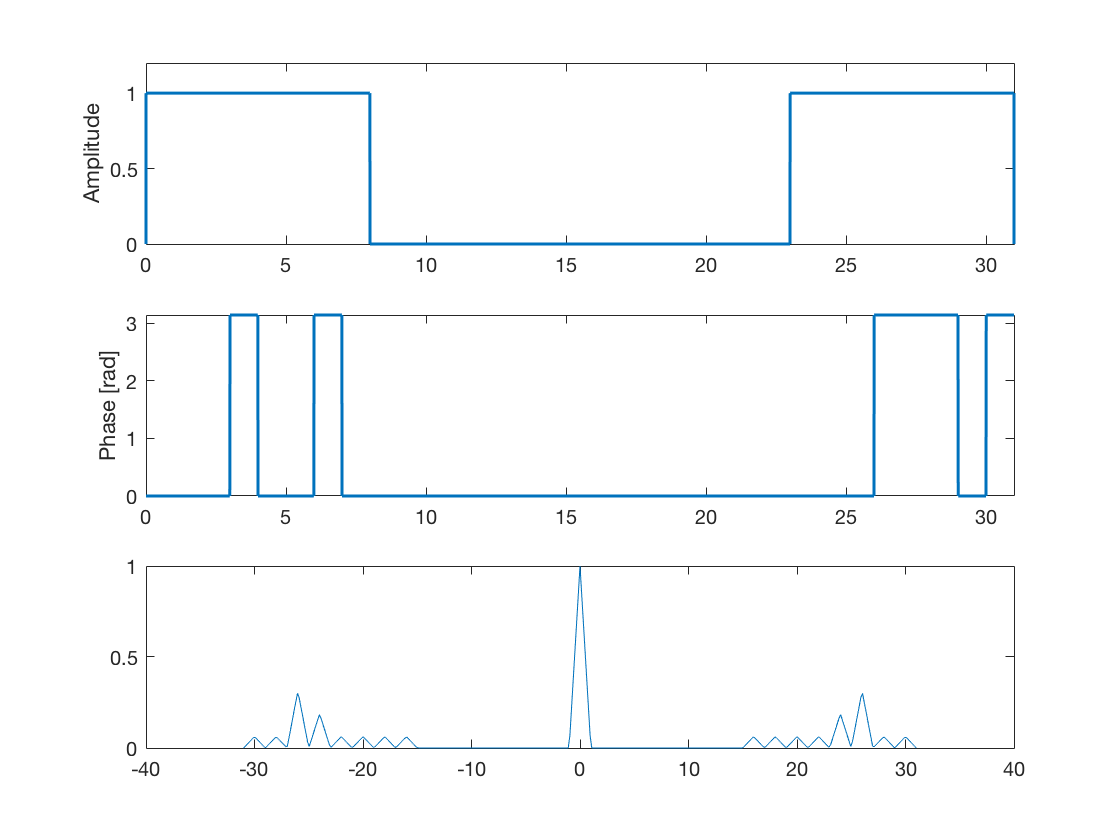
\includegraphics[width=\textwidth]{images/compl8_3}
    \caption{Complementary Coding}
    \label{fig:complCodingProps}
  \end{minipage}
  \hfill
  \begin{minipage}[b]{0.45\textwidth}
    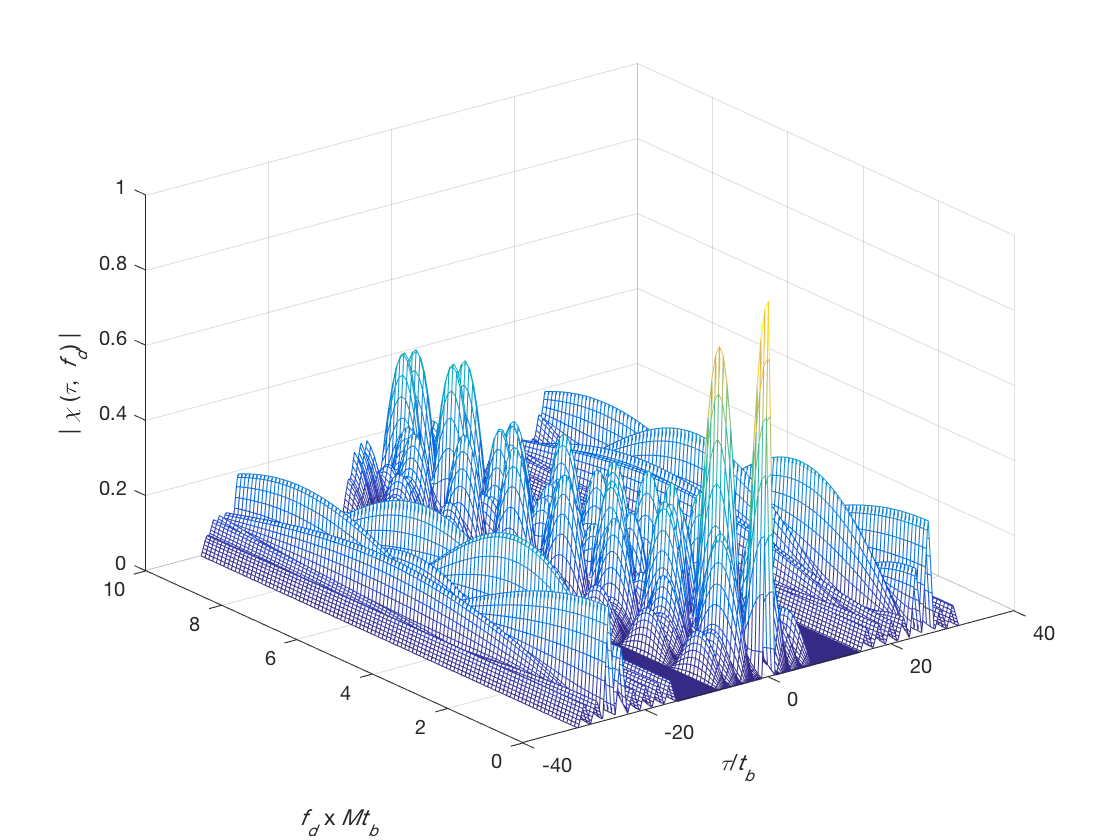
\includegraphics[width=\textwidth]{images/compl8_3D}
    \caption{Ambiguity Surface}
    \label{fig:complCoding3D}
  \end{minipage}
\end{figure}

Again, as stated in chapter \ref{subsec:props}, a high frequency resolution can be obtained by increasing the pulse width, at the expense of range resolution. This can be seen very good in a single long pulse, c.f. figures \ref{fig:longProps} and \ref{fig:longTop} , or also in the Barker Coding with length 2, but to a less extent.

In figure \ref{fig:longTop} one can see very easily, that the yellow part, corresponding to a higher ambiguity magnitude (c.f. fig. \ref{fig:complCoding3D}), is broad on the x-axis, thus having a low range resolution, but is quite low on the y-axis, corresponding to a narrow dopplerfrequency, thus having a better frequency resolution.


\begin{figure}[!htbp]
  \centering
  \begin{minipage}[b]{0.45\textwidth}
    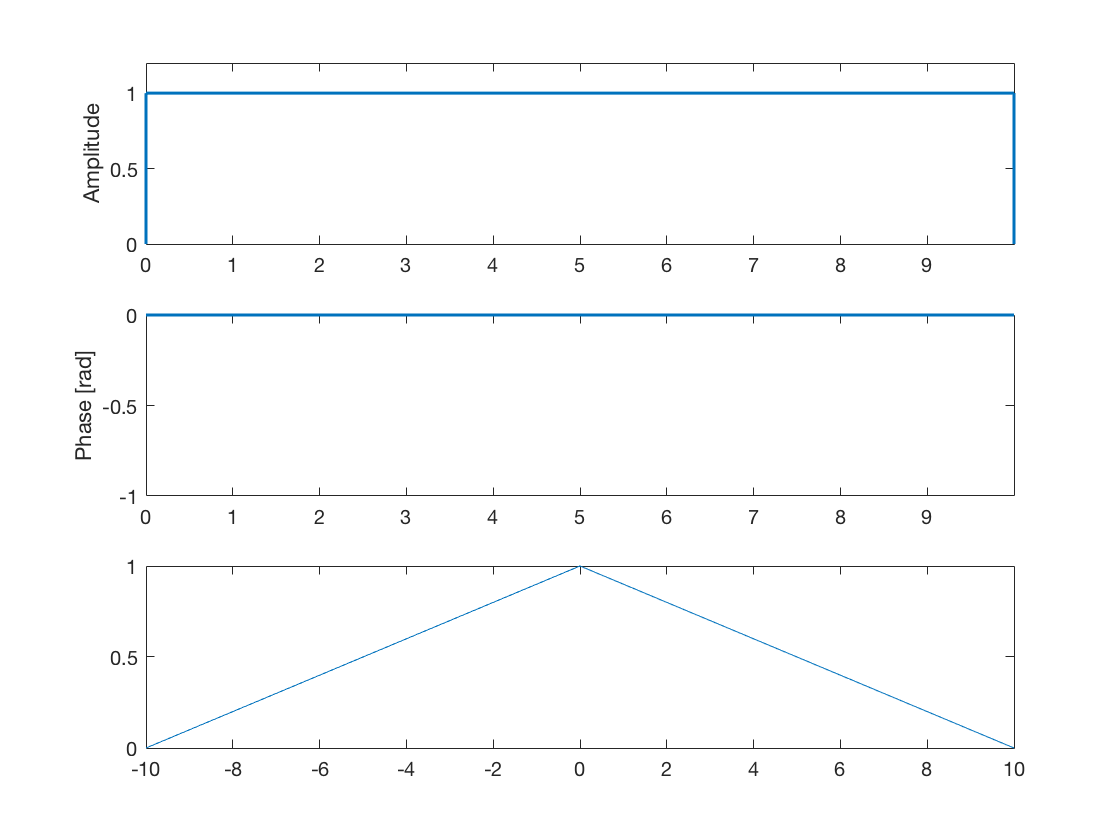
\includegraphics[width=\textwidth]{images/long_props}
    \caption{Long Pulse}
    \label{fig:longProps}
  \end{minipage}
  \hfill
  \begin{minipage}[b]{0.45\textwidth}
    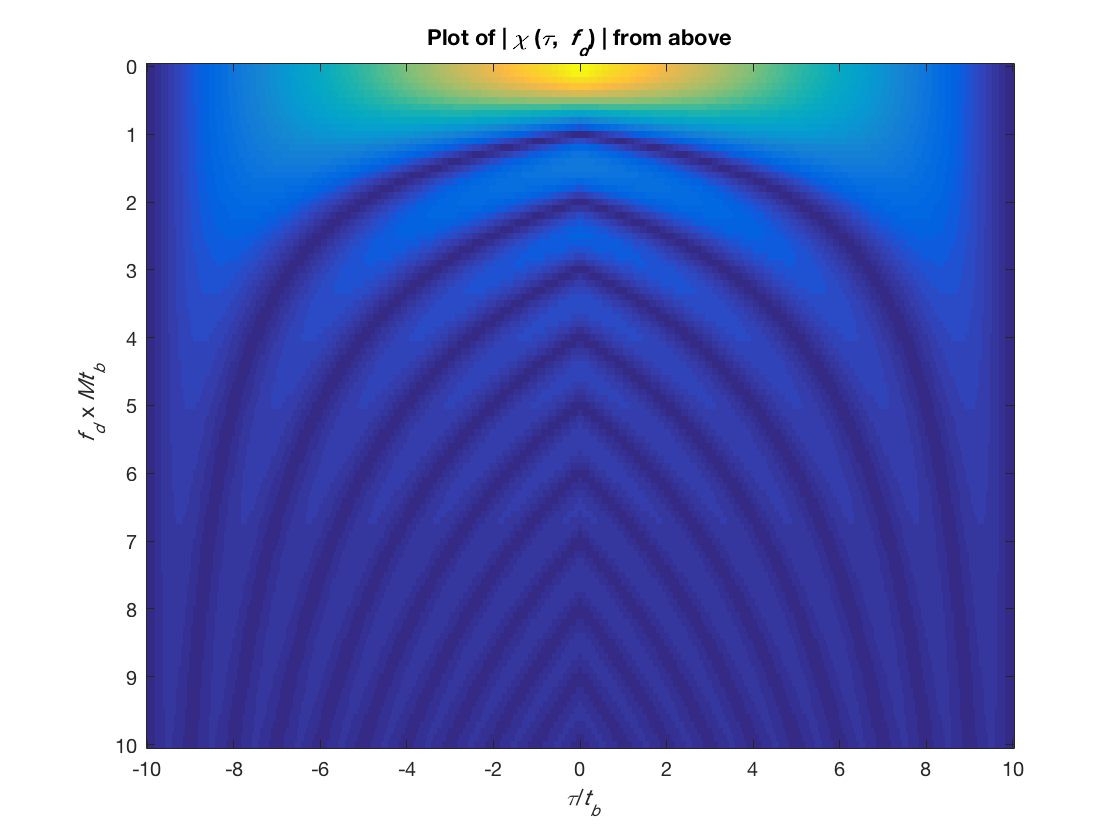
\includegraphics[width=\textwidth]{images/long_top}
    \caption{Top View Ambiguity}
    \label{fig:longTop}
  \end{minipage}
\end{figure}




\subsection{Ambiguities in the diagram}
Ambiguities can be very easily detected in the 3D-Plots of the ambiguity function. Introducing a threshold plane, for example at 0.7 in the normalized ambiguity representation in figure \ref{fig:compl8_side}, one can see that this threshold plane would cut two lobes, the main lobe and one sidelobe. This results in two distinct Ellipses or Circles in the threshold plane. These two distinct circles are ambiguous, since the target doppler and range can not be determined properly.\\
If we set the threshold plane to e.g. 0.9, only one circle is cut out of the threshold plane, thus one has not two distinct ambiguities, but only an area. This area, which is also kind of ambiguous, is still better then two distinct areas, since one can narrow down the range and doppler frequency, which one can not do properly if one has two distinct areas.


\begin{figure}
	\centering
	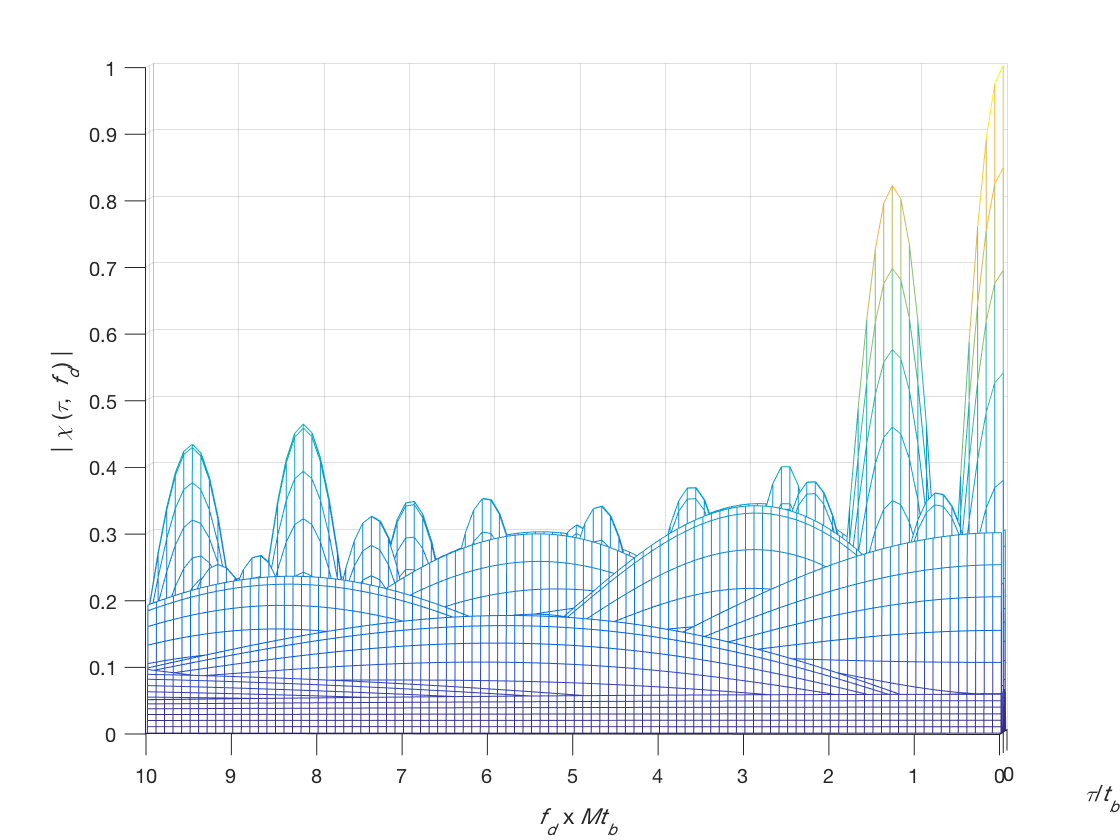
\includegraphics[width=0.8\textwidth]{images/compl8_3D-side}
	\caption{Complementary Coding with length 8, Sideview}
	\label{fig:compl8_side}
\end{figure}


\subsection{Pulse amplitude and pulse width of two radar systems}
Figures \ref{fig:shortTop} and \ref{fig:longTop2} show a short pulse with 1 second and a long pulse with 10 seconds. One can easily see, that the short pulse has a very good range resolution, while sucking at doppler resolution. For the Long Pulse it is vice versa.

\begin{figure}[!htbp]
  \centering
  \begin{minipage}[b]{0.45\textwidth}
    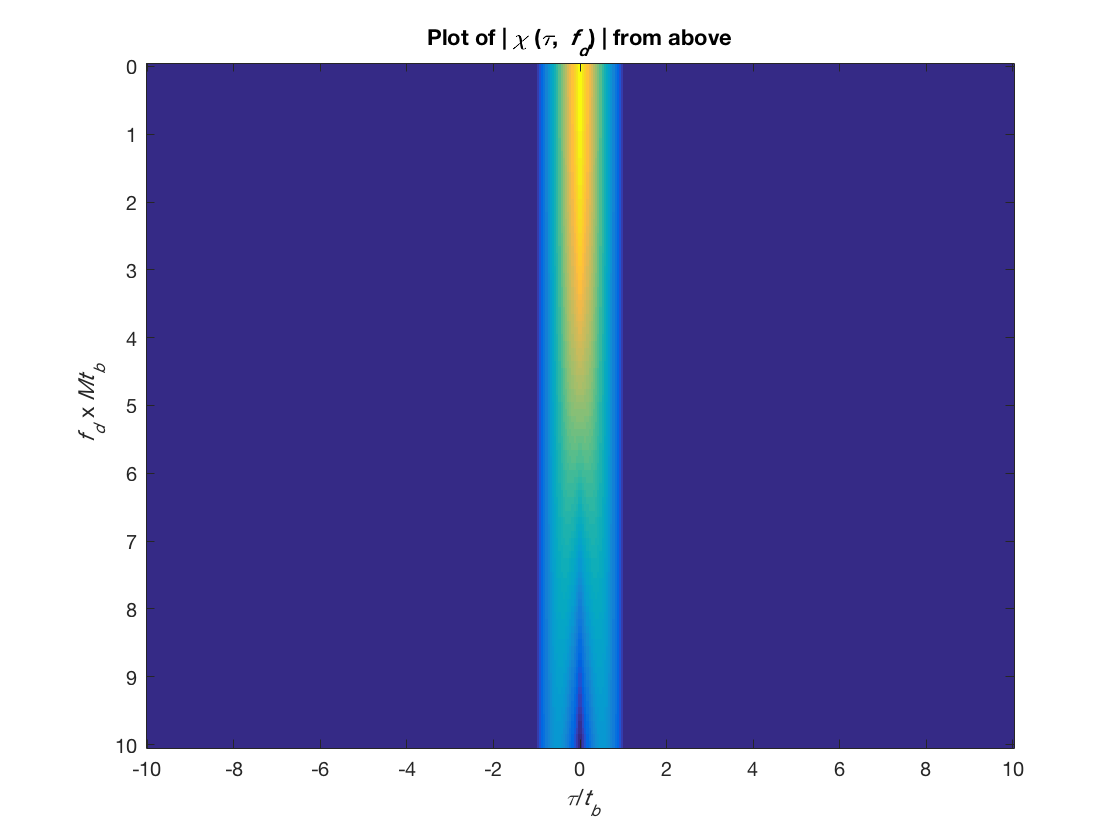
\includegraphics[width=\textwidth]{images/short_1s_top}
    \caption{Short Pulse}
    \label{fig:shortTop}
  \end{minipage}
  \hfill
  \begin{minipage}[b]{0.45\textwidth}
    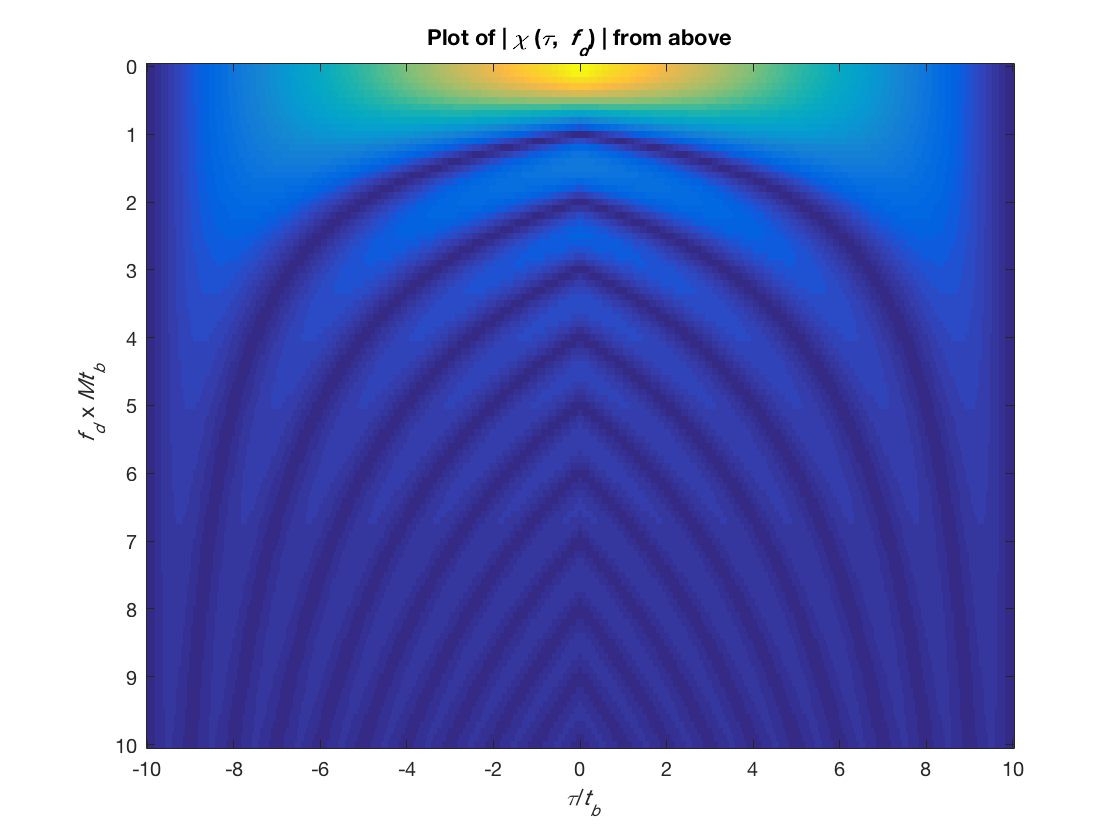
\includegraphics[width=\textwidth]{images/long_top}
    \caption{Long Pulse}
    \label{fig:longTop2}
  \end{minipage}
\end{figure}


\subsection{Comparison of Barker coding and no coding}
Figures \ref{fig:pulse7s_3D} and \ref{fig:7barker_3D} are showing a Barker Coded pulse with barker length 7 and the same pulse width and amplitude as a non-coded pulse (c.f. \ref{fig:pulse7s_3D}).
The Barker Code introduces many more side lobes, but decreases the width of the main lobe, thus leading to a better range and doppler resolution.

\begin{figure}[!htbp]
  \centering
  \begin{minipage}[b]{0.45\textwidth}
    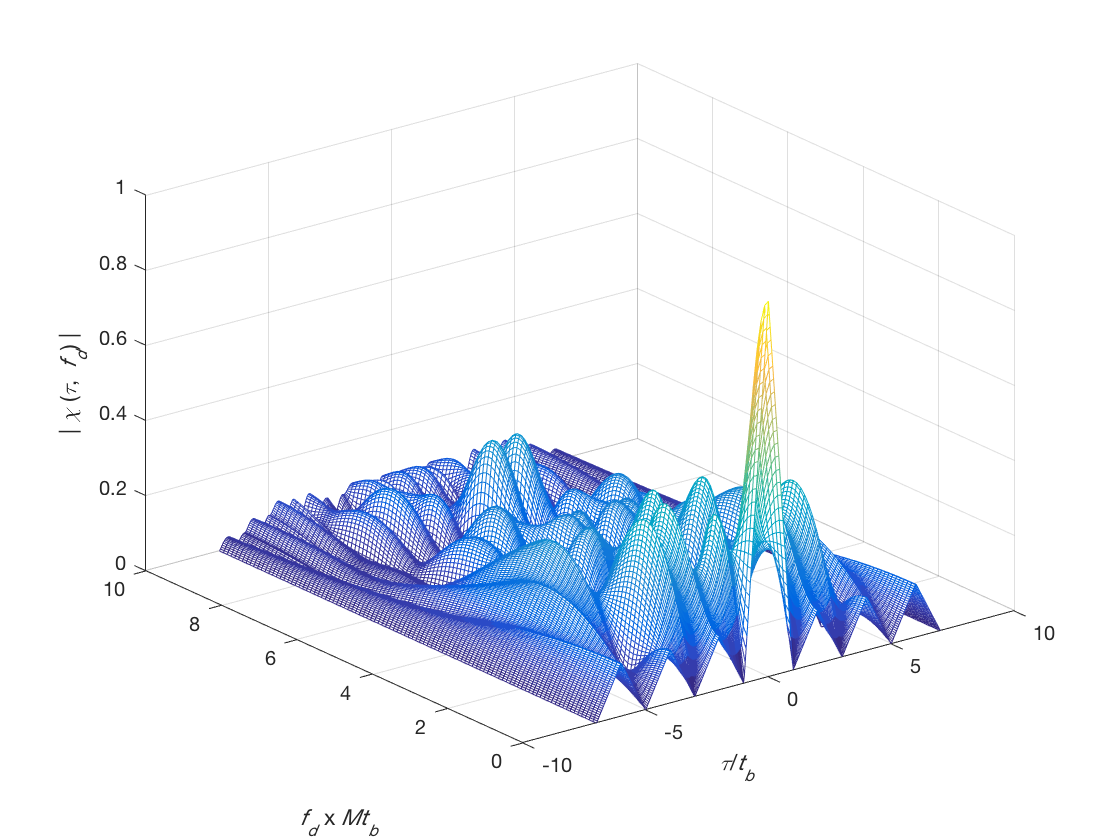
\includegraphics[width=\textwidth]{images/barker7_3D}
    \caption{7 Barker Code}
    \label{fig:7barker_3D}
  \end{minipage}
  \hfill
  \begin{minipage}[b]{0.45\textwidth}
    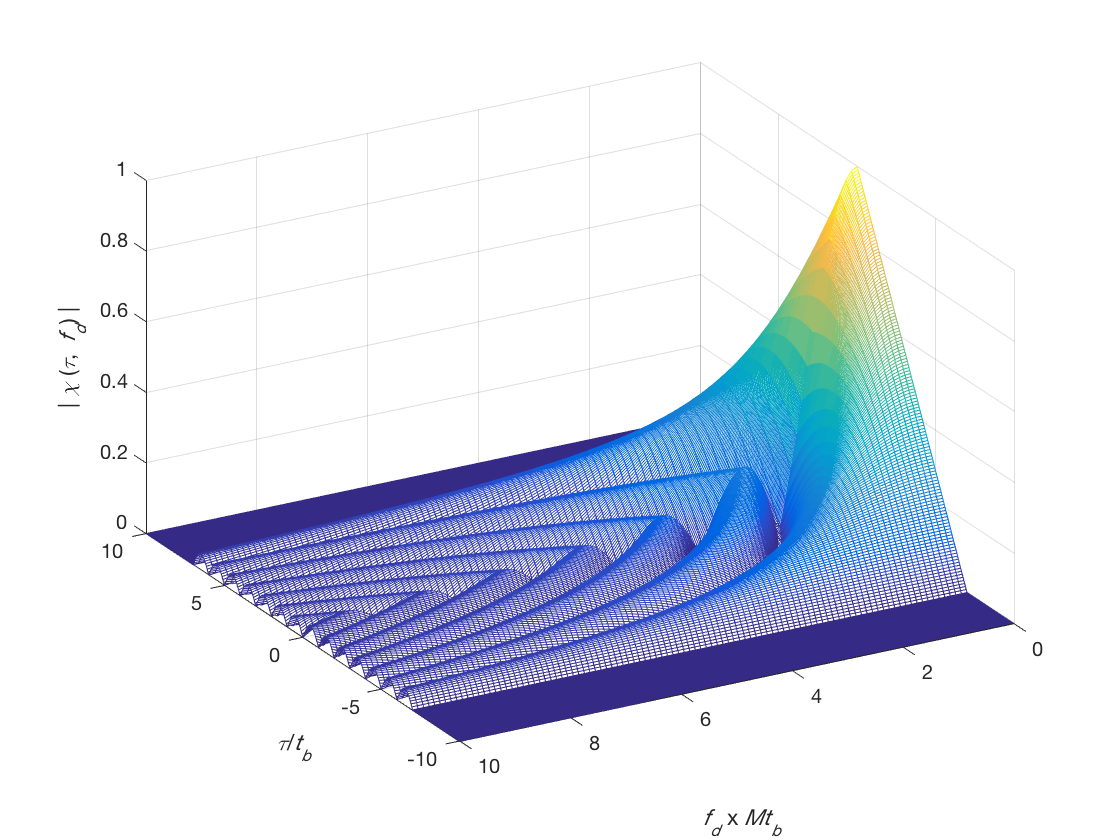
\includegraphics[width=\textwidth]{images/pulse7s_3D}
    \caption{7s Pulse}
    \label{fig:pulse7s_3D}
  \end{minipage}
\end{figure}

\subsection{Comparison of Barker and complementary coding}
Taking into account, that the scaling of the complementary code is different (c.f. lecture notes \citep{enmark:lecture}), one can see that the Barker-coded pulse has more side lobes near the main side lobe, compared to the complementary coding, which might make it harder to have a proper range resolution, e.g. the threshold for SNR has to be higher for the barker-coded pulse.
The Complementary coded pulse introduces much more ambiguities, though, which might be not wanted in certain radar applications.

\begin{figure}[!htbp]
  \centering
  \begin{minipage}[b]{0.45\textwidth}
    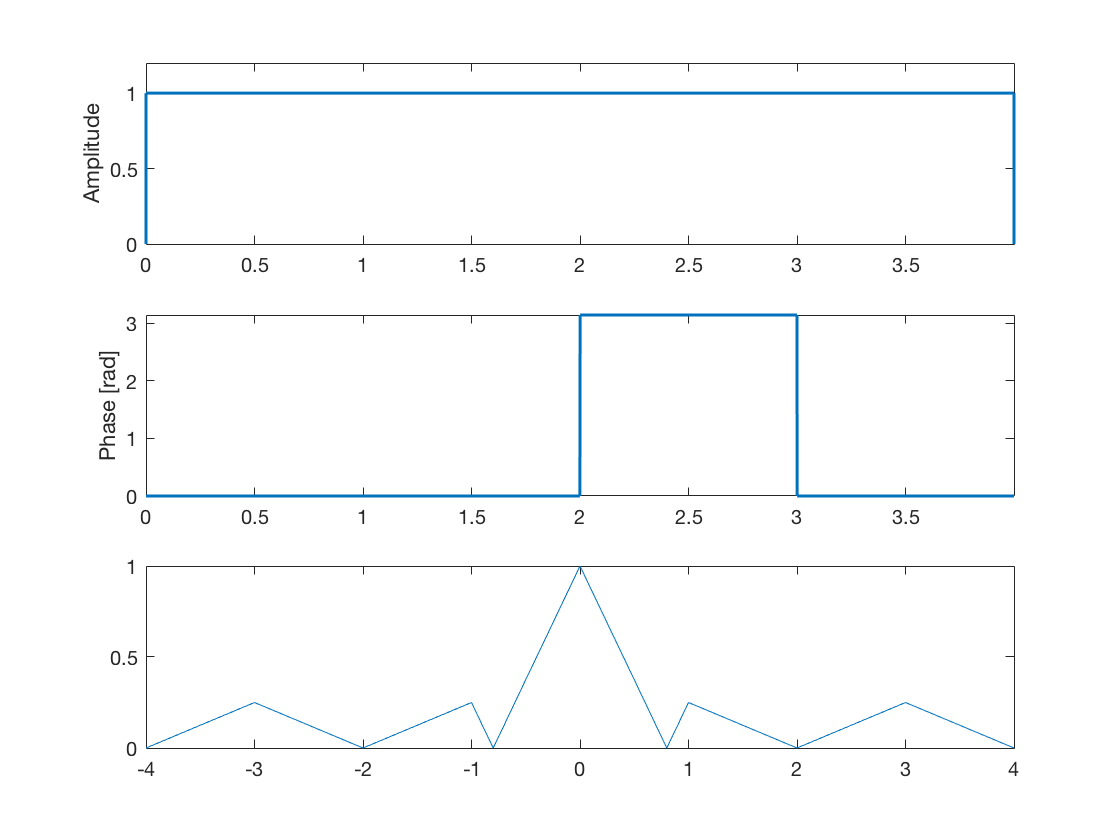
\includegraphics[width=\textwidth]{images/barker4_props}
    \caption{Barker 4 Properties}
    \label{fig:barker4_props}
  \end{minipage}
  \hfill
      \begin{minipage}[b]{0.45\textwidth}
    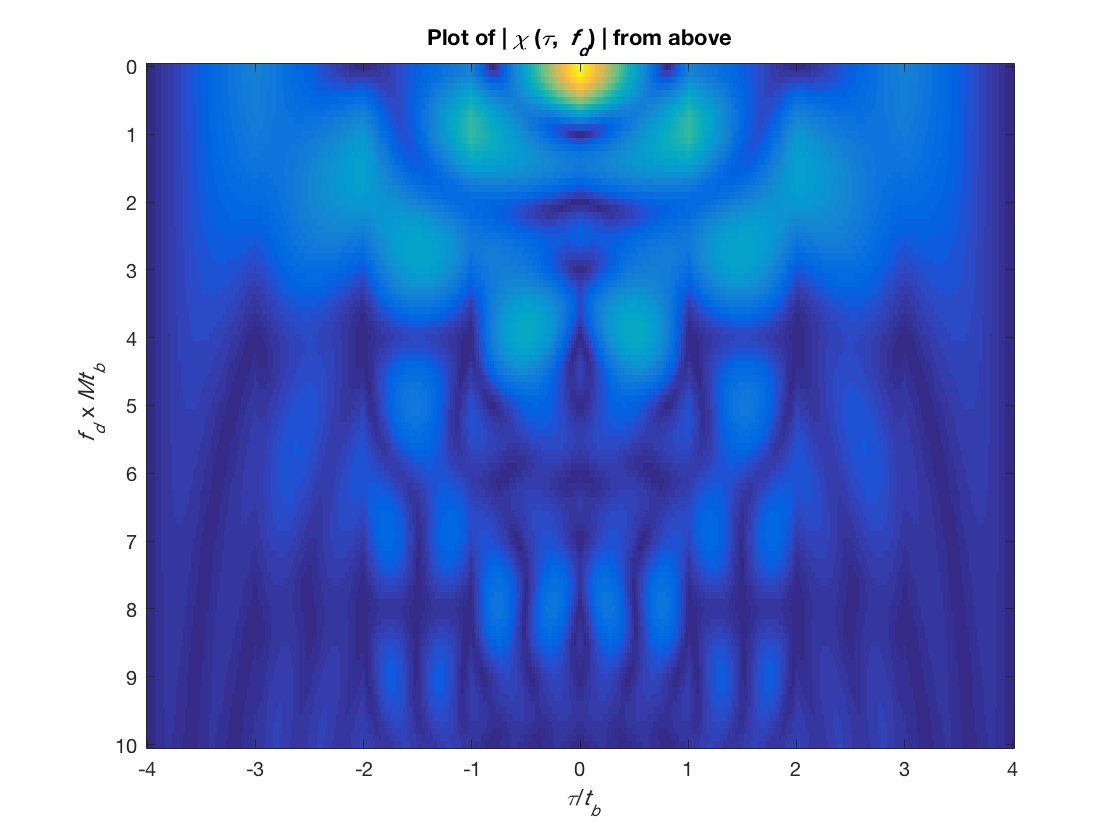
\includegraphics[width=\textwidth]{images/barker4_top}
    \caption{Barker 4 Ambiguity Top}
    \label{fig:barker4_top}
  \end{minipage}
\end{figure}
\begin{figure}
    \begin{minipage}[b]{0.45\textwidth}
    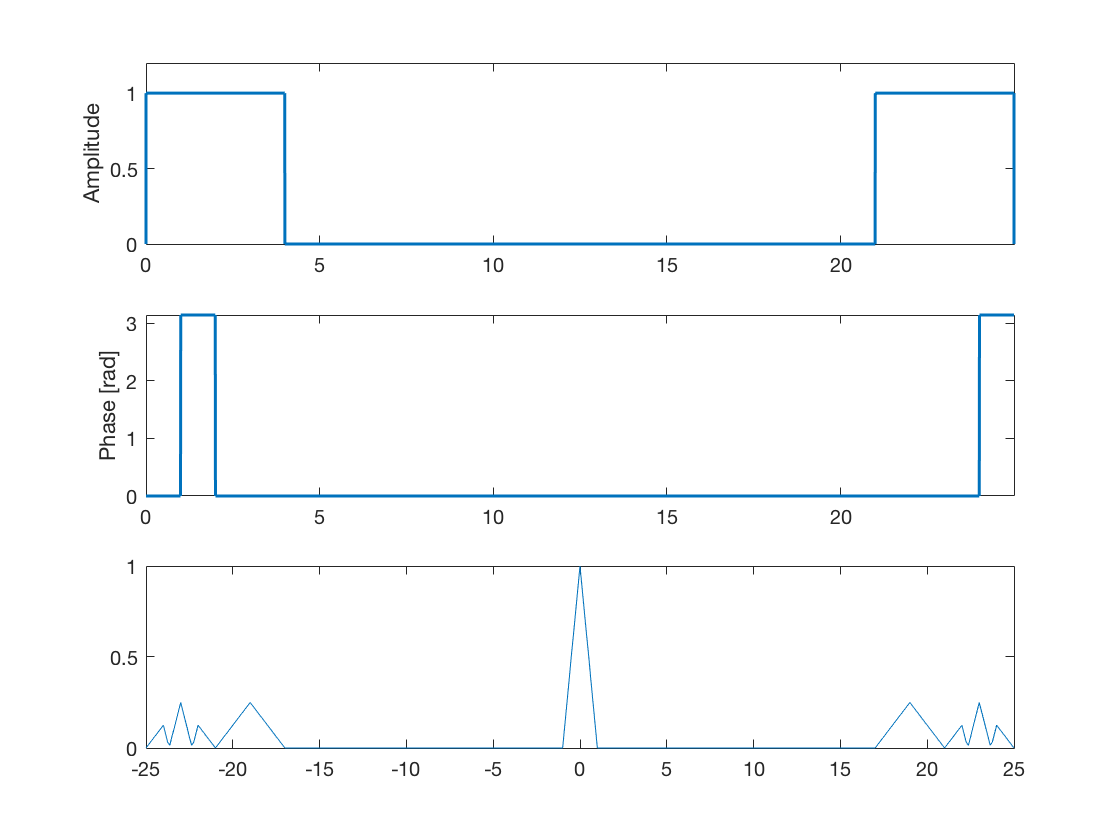
\includegraphics[width=\textwidth]{images/compl4_props}
    \caption{Complementary 4 properties}
    \label{fig:compl4_prop}
  \end{minipage}
 \hfill
  \begin{minipage}[b]{0.45\textwidth}
    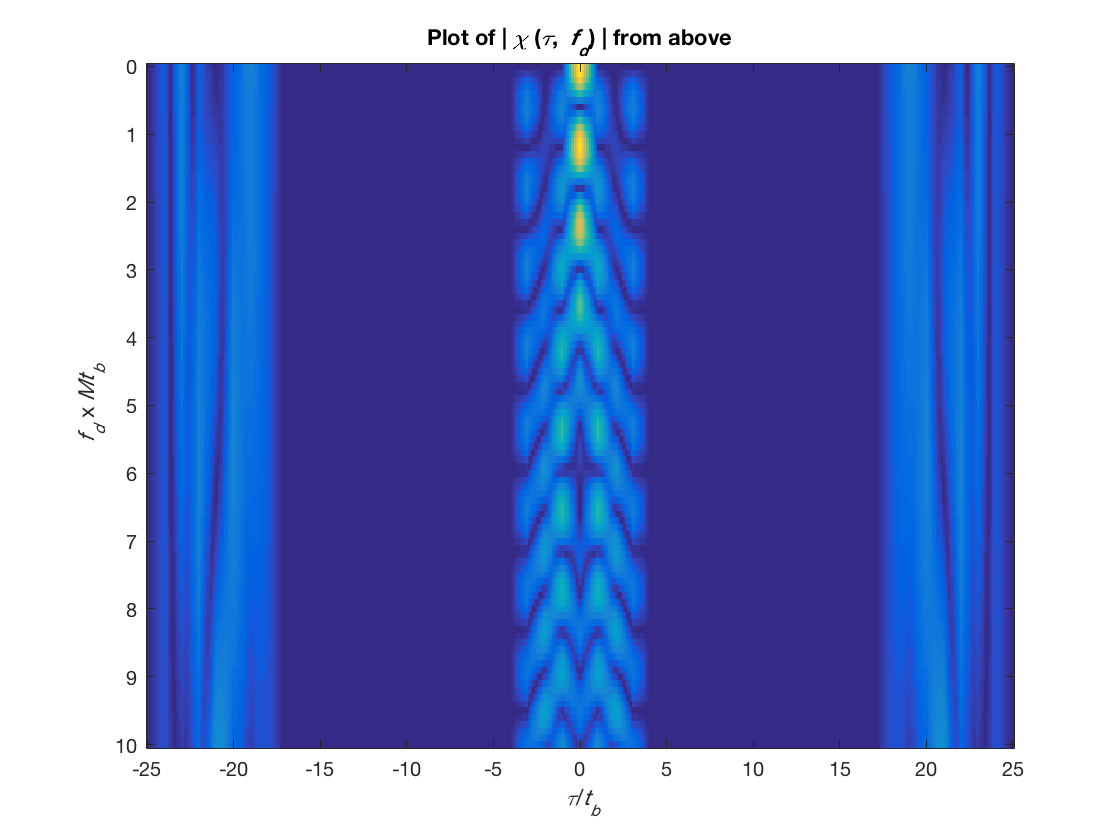
\includegraphics[width=\textwidth]{images/compl4_top}
    \caption{Complementary 4 Ambiguity Top}
    \label{fig:compl4_top}
  \end{minipage}
\end{figure}



\subsection{Comparison of PRN and no coding}

Figures \ref{fig:PRN_props} to \ref{fig:pulse10s_top} show plots of the PRN pulse coding and a non-coded pulse of 10 seconds. Comparing the pulse width of 10s, one can see that the PRN coding has big advantages when it comes to both range and doppler resolution, even though more side lobes are introduced, similar as in the comparison of the Barker 7 and non coding.

\begin{figure}[!htbp]
  \centering
  \begin{minipage}[b]{0.45\textwidth}
    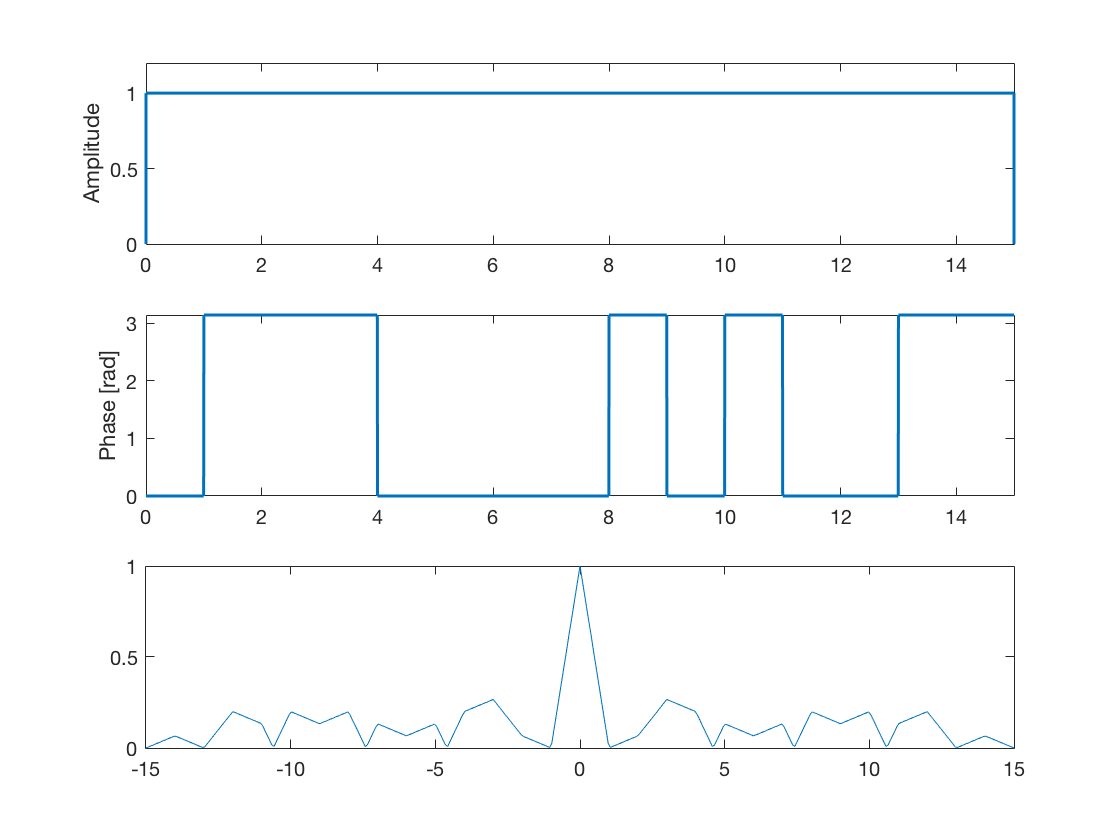
\includegraphics[width=\textwidth]{images/prn_props}
    \caption{PRN Coding Properties}
    \label{fig:PRN_props}
  \end{minipage}
  \hfill
      \begin{minipage}[b]{0.45\textwidth}
    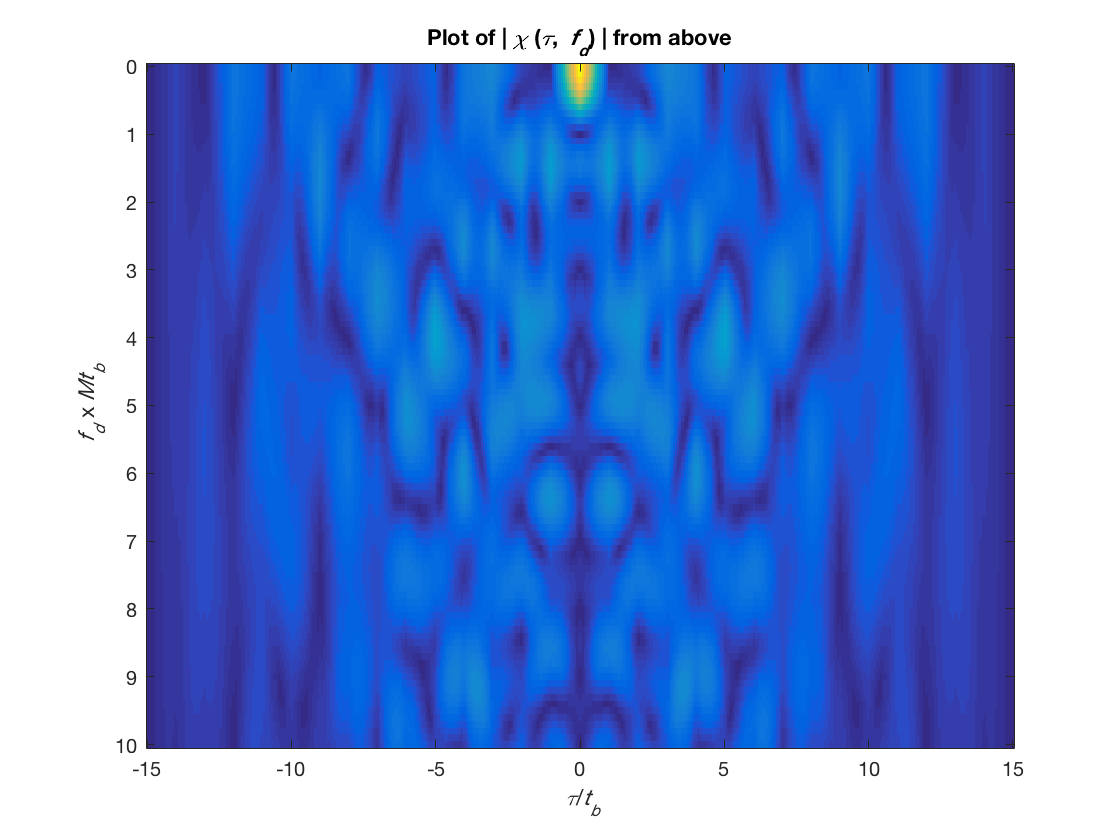
\includegraphics[width=\textwidth]{images/prn_top}
    \caption{PRN Ambiguity Top}
%    \label{fig:7barker_3D}
  \end{minipage}
  \vfill
    \begin{minipage}[b]{0.45\textwidth}
    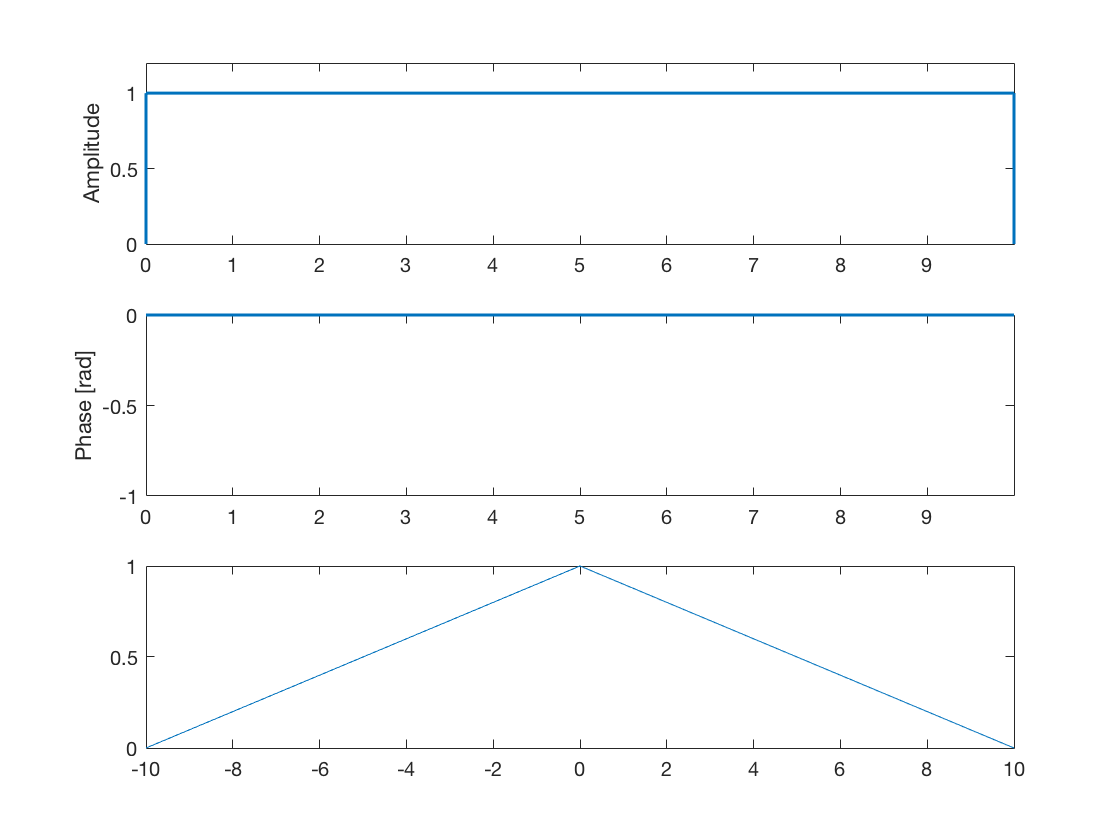
\includegraphics[width=\textwidth]{images/long_props}
    \caption{10s pulse properties}
%    \label{fig:pulse7s_3D}
  \end{minipage}
 \hfill
  \begin{minipage}[b]{0.45\textwidth}
    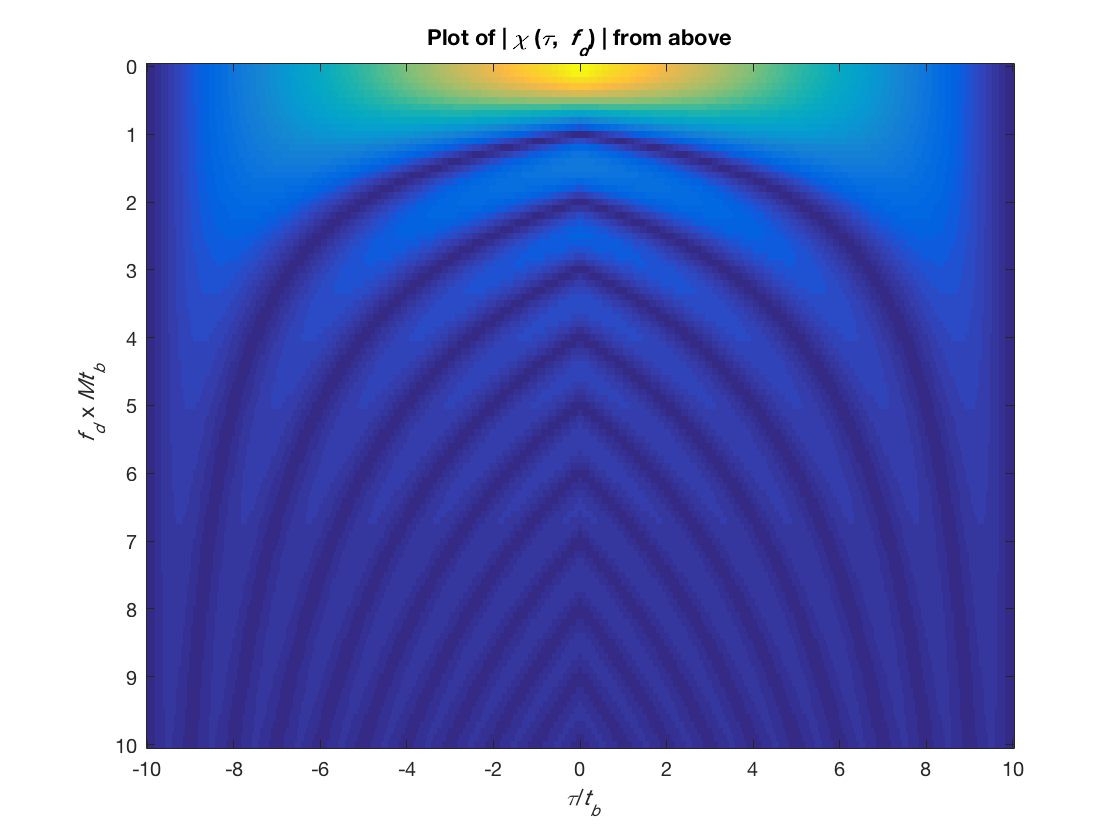
\includegraphics[width=\textwidth]{images/long_top}
    \caption{10s pulse Ambiguity Top}
    \label{fig:pulse10s_top}
  \end{minipage}
\end{figure}



\subsection{Comparison of LFM and no coding}

Again, comparing only the pulse width of 10s, one can see that the LFM coded pulse is much narrower in x-direction, allowing a better range resolution than the non-coded pulse. The Doppler frequency resolution, however, is very similar, or a little bit worse than in the non-coded pulse, c.f. fig. \ref{fig:lfm_top} and \ref{fig:pulse10s_top}.

\begin{figure}[!htbp]
  \centering
  \begin{minipage}[b]{0.45\textwidth}
    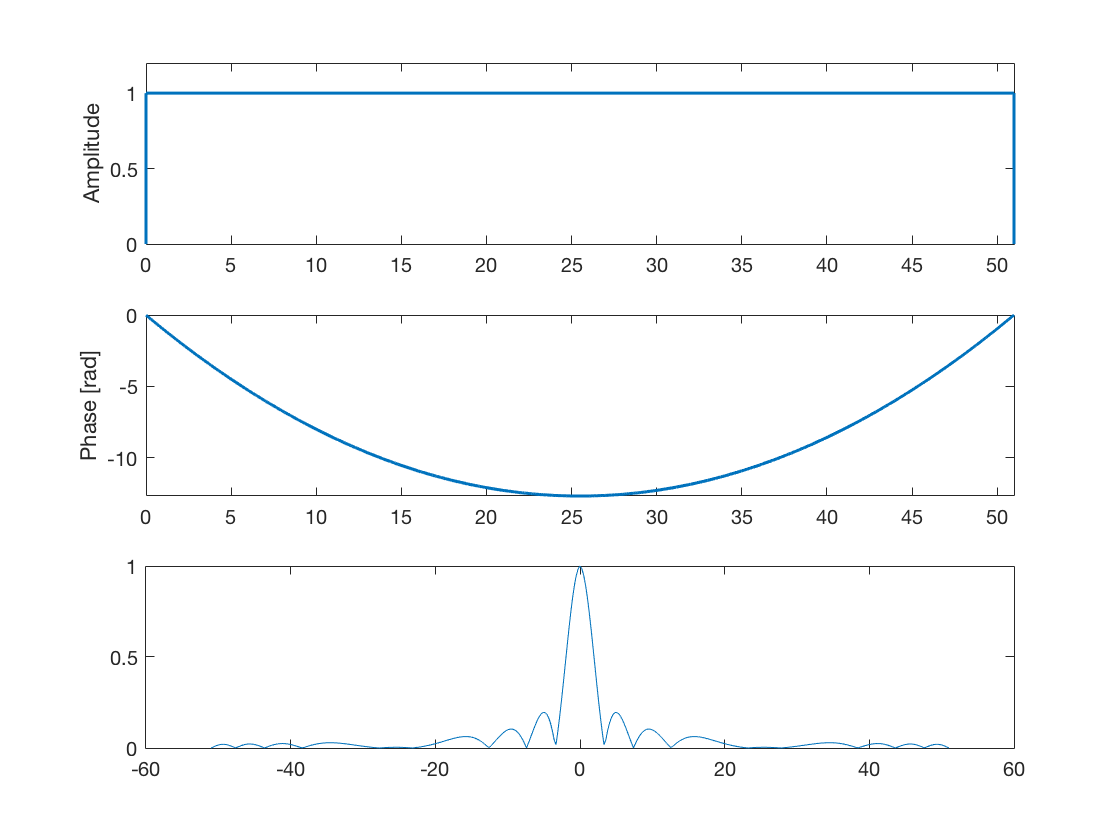
\includegraphics[width=\textwidth]{images/lfm_props}
    \caption{LFM Coding Properties}
    \label{fig:lfm_props}
  \end{minipage}
  \hfill
  \begin{minipage}[b]{0.45\textwidth}
    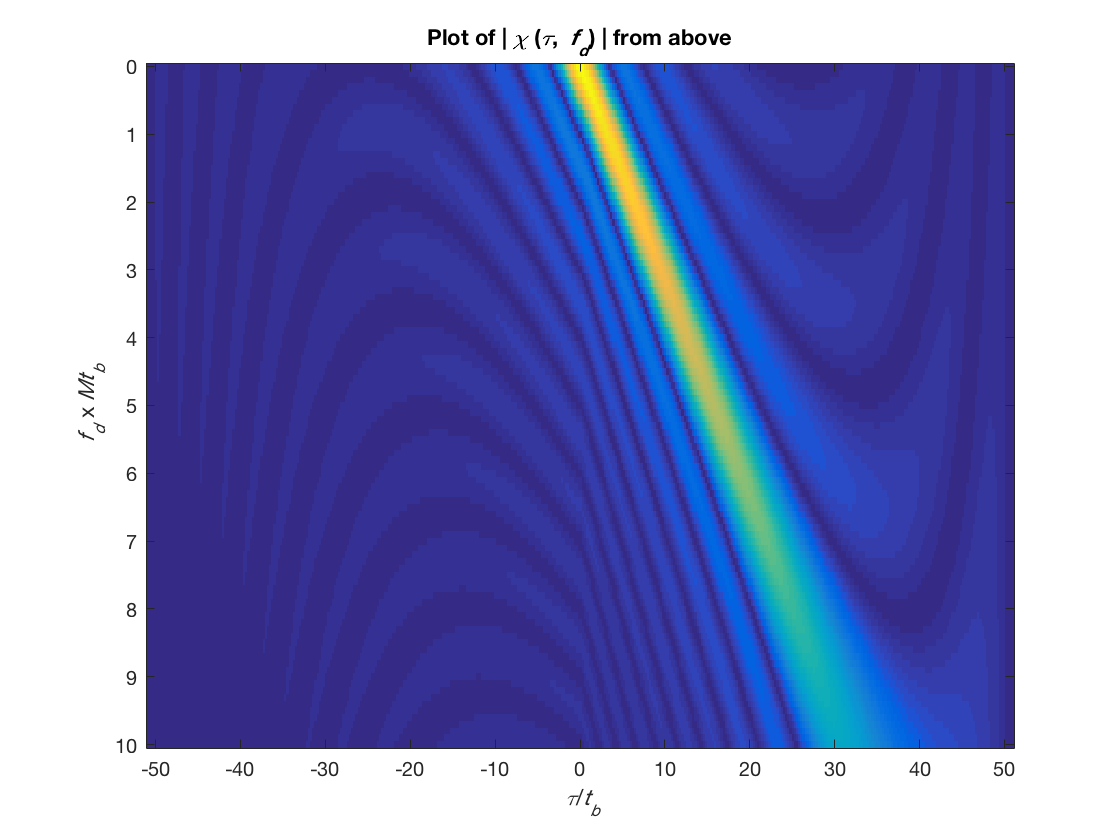
\includegraphics[width=\textwidth]{images/lfm_top}
    \caption{LFM Ambiguity Top}
    \label{fig:lfm_top}
  \end{minipage}
\end{figure}


%%%%%%%%%%%%%%%%% TASK 2 %%%
\section{Reduction of effective height resolution}

\subsection{Signal-to-noise ratio as function of time}
Using the provided datasets, captured on 28th February 2006, the Signal-to-Noise ratio is plotted against altitude and local time. The associated MATLAB-Code can be found in Appendix \ref{apx:matlab}. The Code used is similar to the one used in \textit{Problem 2 - General Radar Theory} to plot SNR against altitude and time.

\begin{figure}
	\centering
	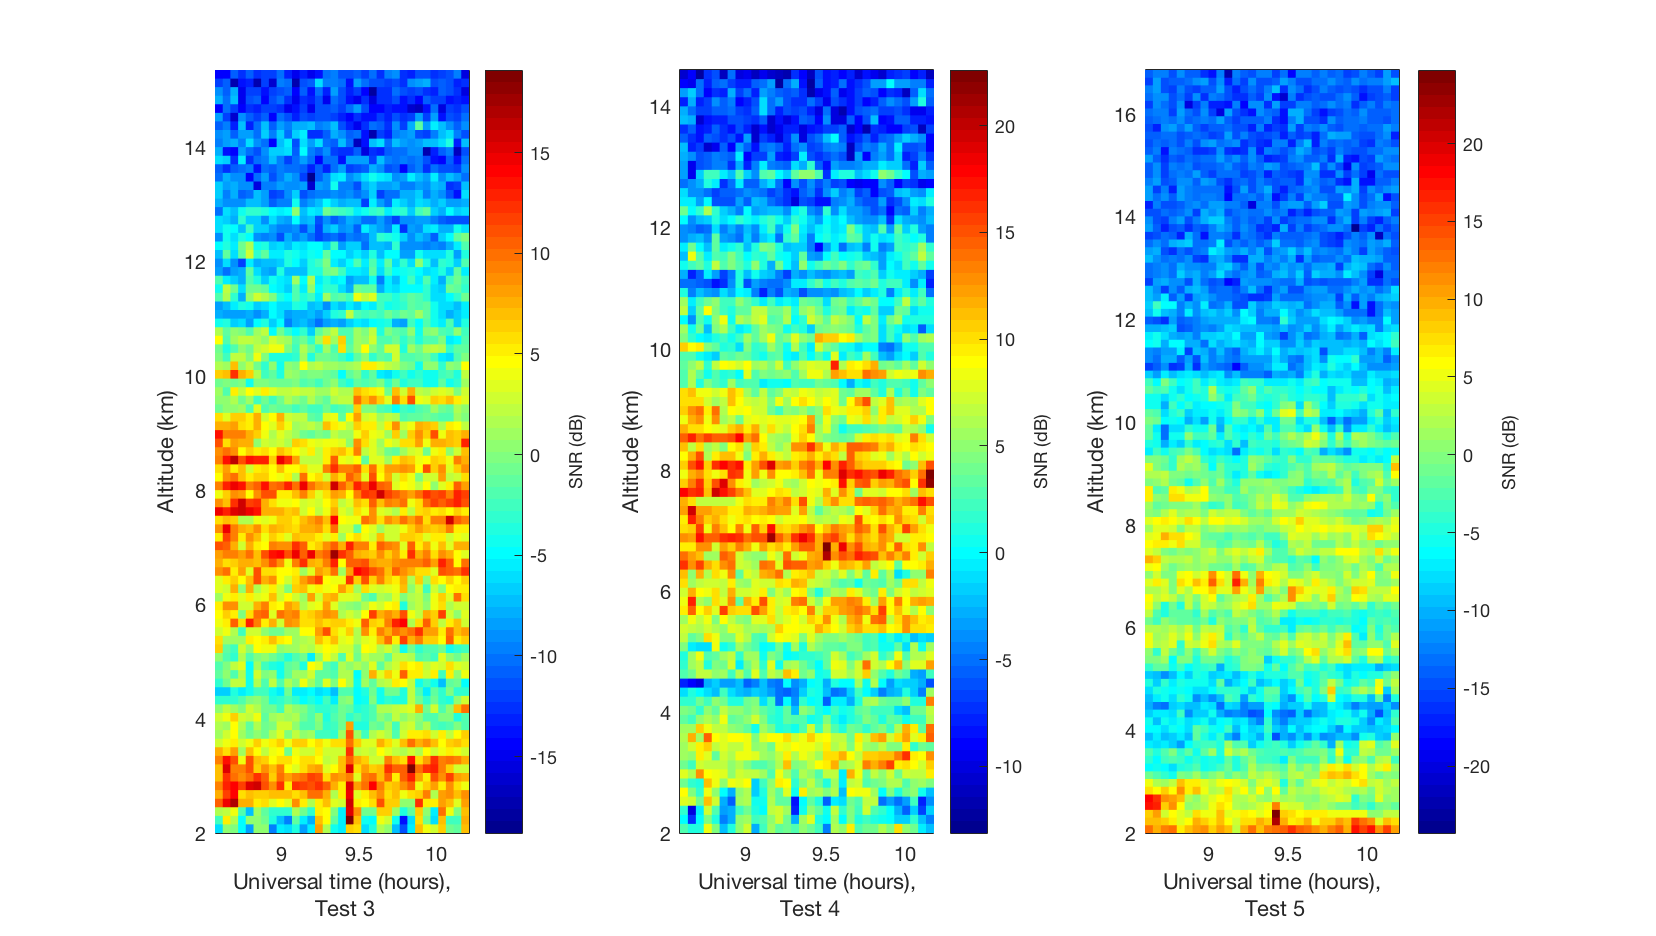
\includegraphics[width=0.9\textwidth]{images/task2_snr_plot}
	\caption{SNR against altitude and time for each dataset}
	\label{fig:snr}
\end{figure}

Each dataset for the three tests contains radar data with different coding techniques; test 3 has Barker coding, test 4 complementary coding and test 5 has uncoded data. \newline



\subsection{Scientific usability of obtained data plots}
As one can easily see in Fig. \ref{fig:snr}, test 4, the complementary coding has the highest SNR compared to the other two tests. Thus it seems that this dataset can give the most detailed view of the atmosphere, concerning.
Although one could argue, that the SNR is almost too high, since the region between 5 and 10 km is almost. \todo{what to write here?}
\subsection{Dynamical state of the atmosphere}









